\section{Design Rationale: Educational use cases}


\begin{figure}
\begin{center}
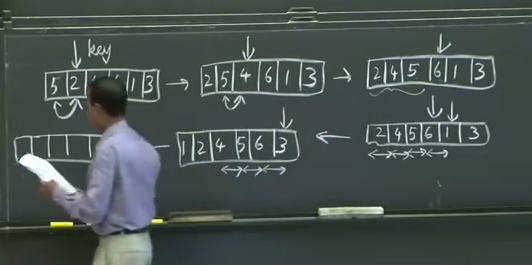
\includegraphics[width=0.7\columnwidth]{img/6006/insertion.png}
\end{center}

\caption{An algorithms instructor traces the operation of insertion sort 
on a concrete example of a list by drawing storyboard snapshots.}

\label{fig:6006-insertion}
\end{figure}


CodeInk's design is inspired 
by  the actions of instructors and by best practices
identified in educational psychology.

One such practice~\cite{Lister2004} found that a student's ability to trace code is a
prerequisite for being adept at problem solving and writing code, suggesting that CS courses should ``first teach systematic tracing as a base
skill, then allow students to build [\ldots]\ upon that''.
% found that students in introductory programming courses could not
% consistently demonstrate an understanding of code by manually tracing
% it. The researchers noted that ``even when our principal aim is to
% teach students to write code, we require students to learn by reading
% code''

We also noted that instructors often start explaining algorithms by
tracing code on concrete examples (\fig{fig:6006-insertion}), rather
than explaining the algorithm in the general case or drawing flow
control.  Instead, they unfold the loops and branches of an
algorithm's pseudocode into a linear sequence of steps.
%%% POSSIBLY PUT BACK IN THE TEXT COMMENTED OUT BELOW?
%%%
% This approach is in line with findings that students need to see multiple
% examples of an algorithm's behavior to build their
% understanding~\cite{Vainio2007}.

In response to both of these observations, CodeInk targets the task of
tracing algorithms behavior on concrete examples, enabling students to
practice tracing examples in an engaging, interactive environment.
The student has the freedom to explore an algorithm's behavior,
perhaps making mistakes along the way.  CodeInk records every action
the student makes, providing a basis for targeted
feedback~\cite{Balzer1989} on both the final answer and the process by
which the student reached their answer.

We further noted that algorithm explanations typically occur at a high
level of abstraction, using pseudocode and diagrams rather than
language-specific code. This abstracts away language-specific details,
a lesson incorporated in CodeInk's goal of enabling the illustration of
algorithm behavior by direct manipulation of data structure diagrams.

Finally, CodeInk uses the visual vocabulary common to programmers, e.g., 
lists drawn as a row of boxes (\fig{fig:6006-insertion}), trees and graphs
drawn as circles connected by arrows. Values are drawn as a number
within or adjacent to each object (Figure 3).\footnote{All examples in our system so far
use numerical data.}

%Also, according to cognitive load theory, novices can learn better by watching
%experts solve problems that would be too difficult for novices to solve on
%% their own~\cite{Linn1992, Sweller1985}. The instructor's worked examples give
%% students
%an opportunity to get the gist of an algorithm, before they attempt to trace it
%on their own. 



\begin{figure}
\begin{center}
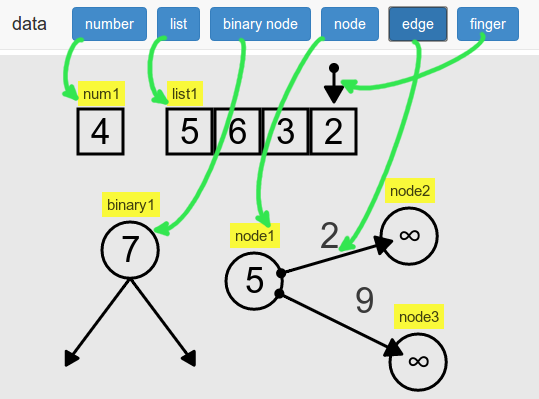
\includegraphics[width=0.8\columnwidth]{img/visual-vocabulary.png}
\end{center}

\caption{CodeInk's visual vocabulary and data palette, located at the
top of the interface. The green arrows are for illustration, and
show how the user can drag data structures (numbers, lists, binary tree
nodes, graph nodes, edges) and visual fingers onto the stage.}
%% strongly suggest getting rid of green arrows; they are confusing and not
%%% needed. Say instead: ``Each of the data structure types at the top can be dragged onto the stage.��
%% also: later in the paper we talk about �the canvas� rather than �stage�.
%% Pick one term and stick to it.
\label{fig:visual_vocab}
\end{figure}


\begin{comment}
Instructors add to this vocabulary using arrows and colors. Arrows are
interchangably used to show transitions between storyboard frames, or to point
to the current focus of the algorithm (\fig{fig:6006-insertion}). The former is
an artifact of the need to draw snapshots when using blackboards, while the
latter is an important visual cue for following the algorithm's progress. Colors
are also used to visualize state; for example, to mark graph nodes as visited,
they are filled with a different color. CodeInk's visual vocabulary includes
\emph{fingers}, which can be attached to any on-screen object, and a \emph{fill}
gesture (explained later) that can be used to color a data structure.
\end{comment}


% Show your work

%Finally, students eventually need to learn to write algorithms in a real
%programming language. CodeInk provides a mapping from visual data
%structure changes to lines of Python code. This serves as a form of
%instructional scaffolding~\cite{Pea2004} to help students acquire
%basic programming skills.

\begin{comment}

CodeInk supports three main educational use cases:

\begin{itemize}\itemsep0pt

\item Instructors can easily create algorithm explanations that can be
used in a live class or disseminated online.

\item Students can step through instructor-created explanations to learn
both the algorithms and basic Python constructs, such as list
manipulation operators.

\item Students can solidify their understanding by tracing an algorithm
on new input data. CodeInk records all user interactions, which enables
instructors to give targeted feedback~\cite{Balzer1989} on the student's
problem-solving process.

\end{itemize}

\end{comment}

